% Copyright (c) 2008-2009 solvethis
% Copyright (c) 2010-2011 Casper Ti. Vector
% Public domain.

\chapter{GRTSEC设计与实现}\label{chap:grtsec_design}
	在本节将介绍GRTSEC在GRT2.0系统上的改进,
	\ref{sec:grtsec_overview}小节对总体设计和设计思路进行介绍,
	GRTSEC最核心的改进是对物理层信息进行了支持,提取了物理层信息并提供了物理层信息的编程接口,
	\ref{sec:grtsec_phyinfo_substract}小节介绍物理层信息的提取方法,
	\ref{sec:grtsec_phyinfo_api}小节介绍物理层信息的软件编程接口,
	\ref{sec:grtsec_phyinfo_analyzer}小节介绍用于做物理层信息分析的硬件模块设计,
	\ref{sec:grtsec_phyinfo_extension}小节介绍用户如何得到自定义的物理层信息,
	\ref{sec:grtsec_loopback}小节介绍为提高开发调试的效率,射频通信库模块做的改进。

	\section{总体设计}\label{sec:grtsec_overview}
	GRT2.0在用于WiFi安全研究时主要的问题是嵌入式软件与物理层硬件的交互不便,无法获取到物理层信息,
	也无法对物理层模块进行配置和数据传输。
	针对这个问题,我们在GRTSEC的总体设计上提出以下改进,体现在三方面:
	一是扩展了软硬件协同工作的范围,将物理层也与嵌入式处理器通过总线相连,
	方便用户直接对物理层进行配置,以及从物理层获取数据;
	二是提取了常用的物理层信息并提供给用户软硬件的编程接口;
	三是设计了对物理层信息进行分析的软件代码和硬件模块。
	这样做的好处是WiFi安全的研究者可以方便地从软件端获取常见物理层信息,以及扩展其它的物理层信息,
	并且可以选择由硬件或软件实现自己提出的安全机制,验证其正确性。

	GRTSEC的硬件结构如图\ref{fig:grtsec_hw_design},
	图中block design内为软硬件协同设计的部分,由于暂未有对USB通信库编程的需求,放在block design之外,
	图中Core为原GRT2.0中的嵌入式MicroBlaze处理器,
	Low mac TX、Low mac RX为原GRT2.0中LOW MAC模块的发送端和接收端部分,
	以上为保留的GRT2.0的设计。
	图中PHY TX和PHY RX是将原先的物理层模块移入block design中,与嵌入式处理器通过AXI总线相连,
	射频通信库也移入block design中,
	图中PHY Analyzer模式是GRTSEC新增加的硬件IP,用于对从物理层模块得到的物理层信息进行数据分析,
	并将分析结果反馈给嵌入式软件。
		\begin{figure}
			\centering
			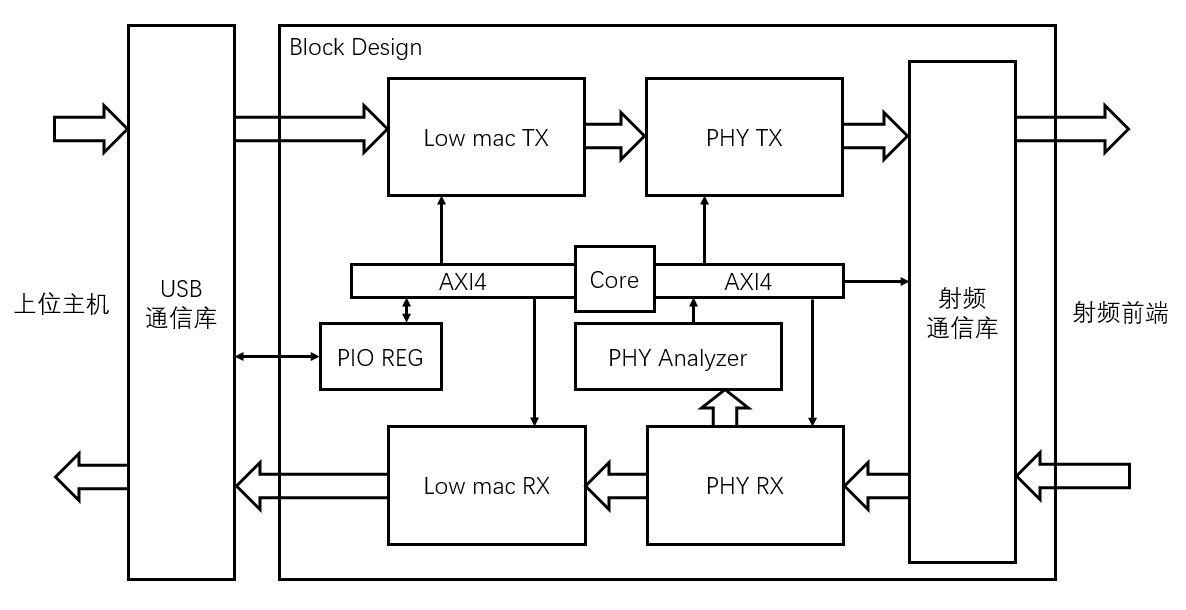
\includegraphics[width=1.0\textwidth]{img/GRTSEC_hw_design.png}
			\caption{GRTSEC硬件模块设计图}
			\label{fig:grtsec_hw_design}
		\end{figure}


	\section{常用物理层信息的提取}\label{sec:grtsec_phyinfo_substract}
	% 在实际的物理层信息提取过程中,我们对物理层信息进行分类,
	% 第一类是随帧物理层信息,每一帧包含一组值,通过前导码(preamble)计算得到,比如CSI、频偏、RSSI、调制方式,
	% 第二类是随符号物理层信息,每一个符号(symbol)包含一组值,每一帧有多个符号,最典型的是导频,
	% 第三类是随采样点物理层信息,每个采样点有一个值,比如星座点偏移向量。
	% 在物理层WiFi安全的研究中,绝大多数使用的是第一类,随帧物理层信息,GRTSEC对这一类物理层信息进行了提取。
	% GRTSEC虽然未提供随符号物理层信息和随采样点物理层信息的接口,但在各个模块中包含有原始信息,用户可自行提取,
	% 参照\ref{sec:grtsec_phyinfo_extension}小节进行扩展。

	在实际的物理层信息提取过程中,物理层信息如CSI、频偏、RSSI、调制方式等,往往是跟随一帧的,
	即接收到的一帧对应了一组物理层信息,这些物理层信息也大多是通过一帧的前导码(preamble)计算得到。
	对于物理层信息的提取,我们面临着两个问题,一是物理层信息的帧对齐问题,二是精确接收时间问题。
	物理层信息的帧对齐问题是指当软件MAC层收到一帧时,如何获取该帧对应的物理层信息,
	假如此时去物理层取,有可能下一帧已经到来,得到的是下一帧的信息,也有可能当前帧的物理层信息尚未计算完毕,得到的是上一帧的信息。
	精确接收时间问题是指软件MAC层收到一帧时如何知道该帧的精确到来时间,
	在TMC 10\cite{tmc10clock}这篇文章中提出利用帧到来时间作为计算硬件指纹的依据,到来时间必须精确到us级别,
	但软件代码的执行会受操作系统调度的影响,即使是嵌入式软件,也会受中断的影响,无法精确的标定帧到来的时间。

	对于物理层信息的帧对齐问题,我们采用三级缓存的方法。
	当物理层收到一帧,各个模块通过前导码计算得到物理层信息后,保存在模块内部,与模块的时钟对齐,称作模块内缓存。
	SIGNAL字段在前导码的后面,当此帧的SIGNAL字段被正确解出,且LOW MAC准备好接收下一帧时,物理层会通知LOW MAC模块收到了一帧,
	向嵌入式处理器发起一次中断,此时,我们将模块内缓存的物理层信息,经过时钟域转换,在另一组统一时钟的寄存器中缓存,称作物理层缓存,
	这一步的目的是让各个模块可以继续处理下一帧,更新模块内缓存。
	LOW MAC的软件收到中断后,将物理层缓存的物理层信息,存放到与AXI总线时钟对齐的第三组寄存器中,称作AXI缓存,
	处理器通过AXI总线读取AXI缓存的物理层信息,此时读到的即为收到中断的那一帧的物理层信息,
	这一步的目的是让物理层可以向LOW MAC发起下一帧的终端,而嵌入式处理器在一帧之内的后面的任意位置都可以读取这一帧的物理层信息。
	我们将物理层信息缓存在寄存器中,而不是将物理层信息缓存在队列中,因为SIGNAL有可能会解错,嵌入式软件也可能会丢掉中断,
	一旦SIGNAL错误或中断没有被处理,缓存的物理层信息就不会继续被读取,阻塞了队列,队列发生错位。
	假如缓存在寄存器中,发生错误时后面帧的物理层信息会覆盖前面的,不会引起错位。
	图\ref{fig:phy_info_cache}描述了三级缓存的思想。
		\begin{figure}
			\centering
			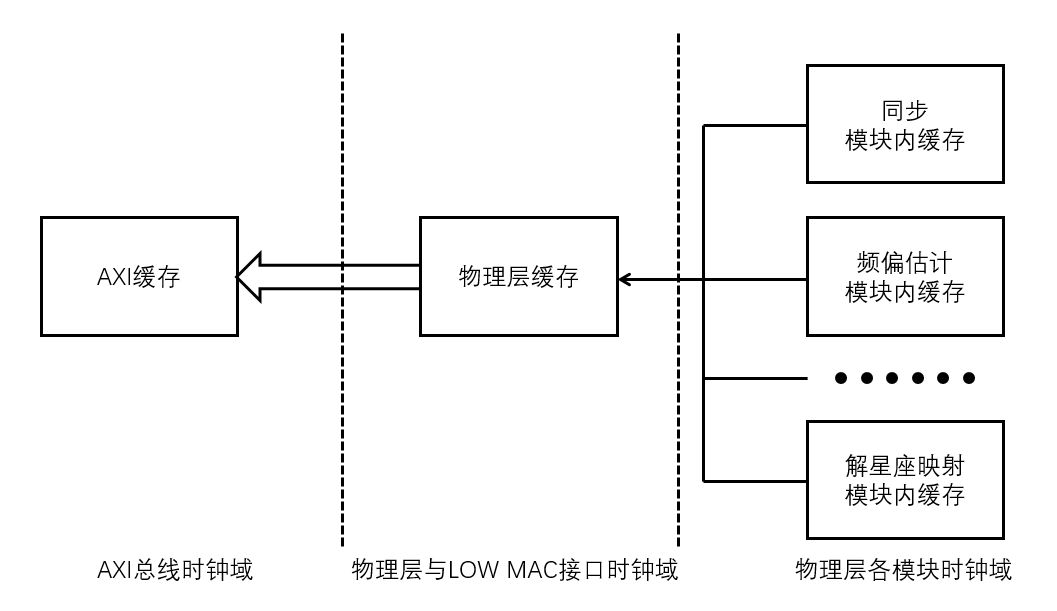
\includegraphics[width=0.7\textwidth]{img/phy_info_cache.png}
			\caption{GRTSEC物理层信息三级缓存示意图}
			\label{fig:phy_info_cache}
		\end{figure}

	采用三级缓存方法的好处是,在保证一帧的数据段与物理层信息保持同步的同时,不阻塞后面帧的接收和数据处理过程,
	并且使用寄存器而不是FIFO,节省了存储空间。

	对于精确接收问题,GRTSEC采用物理层时间戳的方法。首先,我们在物理层与LOW MAC接口处使用一个64位的计数器,每一个时钟周期加一,
	目前此处的时钟频率是100MHz,那么计数器的精度就是10ns。然后,当物理层同步到一帧时,读取计数器的值并保持下来,
	LOW MAC软件通过AXI总线读取保存的计数器值。这种方法是把计数器的值也当做一种物理层信息,采用三级缓存技术进行记录,计数器相当于模块内缓存。
	AXI总线一次读写的宽度是32位,一般而言,读取计数器的低32位寄存器即可,低32位可以记录约43秒的时间间隔,对于超过43秒的时间,则读取高32位寄存器。

	采用物理层时间戳的好处是,用户可以精确地获悉当前帧的相对接收时间,一方面可以单独作为一个物理层信息计算得到时钟偏移\cite{tmc10clock},
	另一方面可以与其他物理层信息进行组合,得到其他物理层信息随时间变化的关系,物理层信息的时变性也具有重要的物理含义。

	接下来介绍几种常用随帧物理层信息的提取方法,具体来说,包括CSI、频偏、RSSI、调制方式。
	在第三章需求分析中我们提到,CSI和RSSI是安全研究中最常用的的物理层信息,频偏在基于身份验证的安全机制中也常常被用到。
	调制方式是指物理层数据处理过程中的信源调制方式,对于802.11协议,调制方式有BPSK、QPSK等,
	调制方式是物理层信息的重要参考,提取方式较为简单,分析物理层帧结构,从信令字段(SIGNAL)可以直接得到。
	而RSSI可以通过FMCOMMS3子板的嵌入式驱动程序得到,我们不需要进行提取,直接提供编程接口。
	以下将分别对CSI和频偏的提取过程进行介绍。

		\begin{figure}
			\centering
			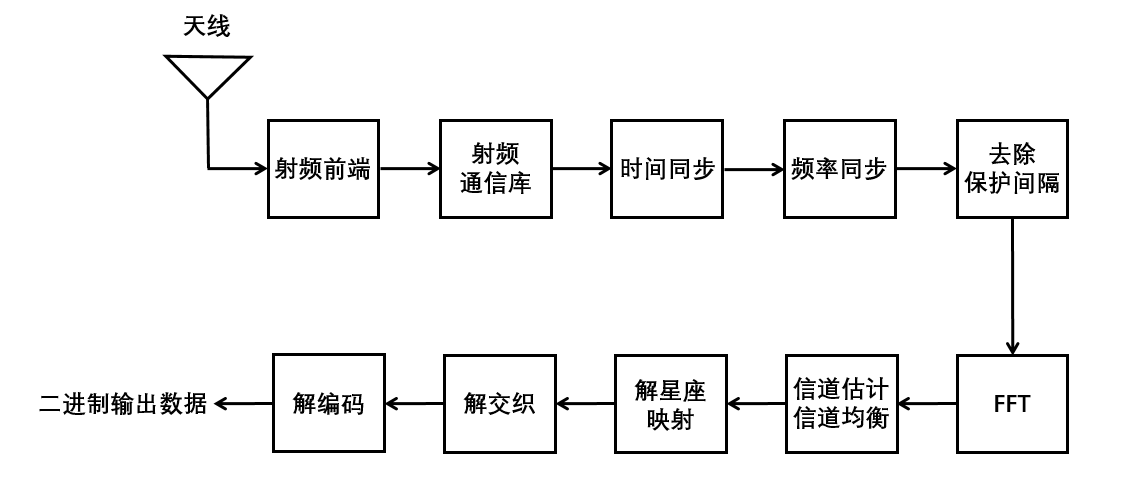
\includegraphics[width=0.8\textwidth]{img/GRT_phy_rx.png}
			\caption{GRTSEC物理层接收端模块示意图}
			\label{fig:GRT_phy_rx}
		\end{figure}

	首先介绍CSI。作为OFDM通信系统,802.11的CSI是指各个子载波当前的信道状况。
	我们假设在一帧的接收过程之内,CSI大致不变,802.11协议也是基于此假设使用训练字段对信道进行估计。
	GRTSEC的物理层接收端模块示意图见\ref{fig:GRT_phy_rx},我们在信道估计模块提取到CSI。
	图\ref{fig:80211_spec_preamble}介绍了802.11a/g物理层训练字段的结构,
	训练字段是发送端发送一段双方已知的序列,接收端根据接收序列来做同步、信道估计等。
	802.11a/g物理层帧结构规定了两个训练字段,先是160个采样点的短训练字,后是160个采样点的长训练字,
	在长训练字后面是80个采样点的SIGNAL字段,里面规定了帧长度和调制方式。
	短训练字以16个采样点为周期,共10个周期,采样点间隔为0.05$us$,用来做AGC(自动增益控制)、时间同步、频率同步等,
	在后面介绍提取频偏和RSSI时会进一步说明。
	长训练字前32个采样点是保护间隔,抽取$T_1$、$T_2$各16个采样点组成的,
	$T_1$、$T_2$是重复的。长训练字用来做信道估计、细粒度的频偏估计。
		\begin{figure}
			\centering
			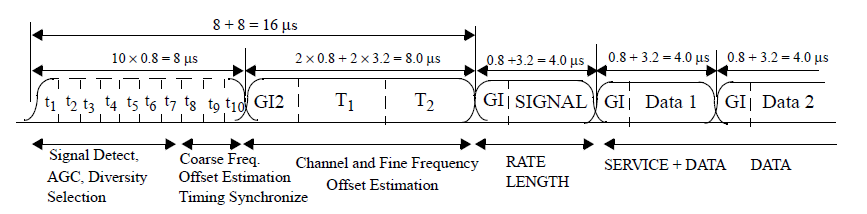
\includegraphics[width=1.0\textwidth]{img/80211_spec_preamble.png}
			\caption{802.11前导码结构}
			\label{fig:80211_spec_preamble}
			\cite{ieee80211}
		\end{figure}

	我们从长训练字中提取CSI。长训练字的采样点为1与-1的序列,如式\ref{fig:80211_lts_sequence},不包含其他值(中间的0为直流分量,不承载信息),
	因此接收值只需转换符号即可得到各个子载波的信道状况。而短训练字中除了1与-1外,还有0和1+j这样的值,不适合提取CSI。
	具体实现时,我们预存长训练字的理论值,与接收到的长训练字进行比较,理论值为-1时对接收值转换符号,理论值为1时不变。
	符号转换后得到52个采样值组成的向量,这个向量便可以代表此帧的CSI。

		\begin{figure}
			\centering
			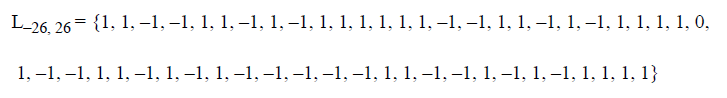
\includegraphics[width=0.9\textwidth]{img/80211_lts_sequence.png}
			\caption{802.11前导码长训练字采样值}
			\label{fig:80211_lts_sequence}
			\cite{ieee80211}
		\end{figure}

	然后介绍频偏的提取。频偏在频偏估计模块中提取,利用短训练字的周期性,具体来说,
	使用短训练字的后64个采样点,即10个周期中的后4个周期,原因有两点,
	一是前面的采样点会受AGC(Automatic Gain Control,自动增益控制)的影响,幅度有波动,
	二是大多数时候从短训练字的中间位置同步到一帧,前面部门有可能同步不到,而后4个周期实践表明是切实可行的。
	我们首先对频偏公式进行变换,此处的推导比第二章更加详细,并结合具体实现。
	假设$k_1$、$k_2$时刻的接收值为$r(k_1)$和$r(k_2)$,理论值为$s(k_1)$和$s(k_2)$,有以下公式:
		\begin{equation}
			\centering
			r(k_1)=s(k_1) \cdot e^{j2 \pi \Delta fk_1 / f_s}
			\label{fig:freq_offseet_rs_1}
		\end{equation}
		\begin{equation}
			\centering
			r(k_2)=s(k_2) \cdot e^{j2 \pi \Delta fk_2 / f_s}
			\label{fig:freq_offseet_rs_2}
		\end{equation}

	其中,$\Delta f$为要求的频偏,$f_s$为采样频率,在802.11a/g中数值为20M,在802.11n中有20M和40M两种情况。
	$r(k_1)$、$r(k_2)$、$s(k_1)$、$s(k_2)$、$f_s$均已知,我们可以通过以下方式求出。
	根据短训练字每16个采样点重复一次的特性可知,当$k_2 = k_1 + 16$时,$s(k_1) = s(k_2)$,
	代入前面的公式,可以推出以下两式:
		\begin{equation}
			\centering
			def: \frac{r(k_1)}{r(k_2)} = A + Bj
			\label{fig:freq_offseet_AB_def}
		\end{equation}
		\begin{equation}
			\centering
			\Delta f = \frac{f_s}{2\pi \cdot 16} \cdot arctan(\frac{B}{A})
			\label{fig:freq_offseet_result}
		\end{equation}

	式\ref{fig:freq_offseet_AB_def}由复数的性质推出,$r(k_1)$、$r(k_2)$都是复数,相除的结果也是复数,
	复数总是可以写成$A + Bj$的形式,其中$A$、$B$为实数。
	式\ref{fig:freq_offseet_result}是将式\ref{fig:freq_offseet_AB_def}代入
	式\ref{fig:freq_offseet_rs_1}、\ref{fig:freq_offseet_rs_2}得出,得到频偏值。

	在具体实现时,我们在硬件中得到$A$、$B$,作为物理层信息传给软件,再由软件计算$arctan$和常数乘法得到频偏。
	硬件计算$A$、$B$时,需要对每隔16个的接收采样点进行相除,
	复数相除$\frac{r(k_1)}{r(k_2)}$可以转化为$\frac{1}{|r(k_2)|^2}r(k_1) \cdot r(k_2)^* $。
	每一个采样点都可以跟它之前的第16个采样点得到一组$A$、$B$,我们对64个采样点得到的64个$A$、$B$进行相加求平均,降低误差,
	最终提取到的物理层信息即为平均的$A$、$B$,分别代表周期性偏移实部和周期性偏移虚部。

	\section{物理层信息软件编程接口}\label{sec:grtsec_phyinfo_api}
	此小节介绍如何将物理层信息从硬件模块提取到软件中。
	GRTSEC的软件代码分为嵌入式软件和上位主机的驱动程序,软件编程接口面临的问题是,
	有研究需要在物理层或LOW MAC层使用这些物理层信息,而另有研究只在主机上进行操作,
	如何满足这两种需求。

	我们采用的方法是嵌入式软件与主机软件的两级编程结构,
	将物理层信息首先提取到嵌入式软件中,提供嵌入式软件的编程接口,然后通过USB通信库将物理层信息传递给主机,
	而不是将物理层信息直接引出到主机驱动程序中。这样做有以下几点好处:
		\begin{itemize}
			\item LOW MAC的控制流程由嵌入式软件实现,用户有可能在LOW MAC中用到物理层信息,
			比如根据物理层信息决定是否回复ACK;
			\item 嵌入式软件包含了与主机驱动程序交互的接口,物理层信息先提取到嵌入式软件中,
			用户决定是否继续将信息继续上传,保持控制流程的集中性;
			\item 硬件逻辑与嵌入式软件的交互方便扩展,倘若用户希望引出其它信息,增加AXI寄存器即可,
			但如果直接引出到驱动程序,还需要对USB通信库的硬件逻辑进行修改,扩展不便,理论上不应对通信库进行过多修改。
		\end{itemize}

	下面介绍具体实现。
	GRTSEC的软硬件之间通过AXI寄存器传递数值,每个寄存器为32位,AXI寄存器定义见表\ref{tab:grtsec_axi_reg_define}。
	与同步相关的寄存器的含义见\ref{sec:grtsec_phyinfo_extension}小节。
	可以看到为了从32位的AXI寄存器传递到软件,我们提供的是原始数据的接口,
	用户得到原始数据后可以选择在嵌入式软件内计算得到最终数据,我们提供了从原始数据得到最终数据的Python示例代码,
	比如由周期性偏移的实部和虚部得到频偏值,
	也可以选择根据原始数据进行处理,很多情况下原始数据比计算结果更有意义。

	\begin{table}[!hbp]
	\centering
	\caption{GRTSEC软件编程接口的寄存器定义}
	\label{tab:grtsec_axi_reg_define}
		\begin{tabular}{|l|l|l|} \hline
		寄存器号 & 读写方向 & 寄存器定义 \\ \hline
		0x00 & W & 请求读取物理层信息 \\ \hline
		0x01 & R & 物理层信息已准备好 \\ \hline
		0x02 & R & 周期性偏移实部,高32位 \\ \hline
		0x03 & R & 周期性偏移实部,低32位 \\ \hline
		0x04 & R & 周期性偏移虚部,高32位 \\ \hline
		0x05 & R & 周期性偏移虚部,高32位 \\ \hline
		0x06 & R & 同步自相关性求和分子 \\ \hline
		0x07 & R & 同步自相关性归一化系数 \\ \hline
		0x08 & R & 同步与短训练字互相关性求和分子 \\ \hline
		0x09 & R & 同步与长训练字互相关性求和分子 \\ \hline
		0x0A & R & 同步互相关性归一化系数 \\ \hline
		0x0B & R & 信令字段,包含帧长度和调制方式 \\ \hline
		0x0C & R & CSI,-21号子载波 \\ \hline
		0x0D & R & CSI,-7号子载波 \\ \hline
		0x0E & R & CSI,+7号子载波 \\ \hline
		0x0F & R & CSI,21号子载波 \\ \hline
		0x10 & R & 时间戳,高4字节 \\ \hline
		0x11 & R & 时间戳,低4字节 \\ \hline
		\end{tabular}
	\end{table}

	\section{物理层信息硬件分析模块}\label{sec:grtsec_phyinfo_analyzer}
	如果物理层安全研究者希望将新安全机制部署在实际通信通信系统中,仅靠软件分析是不够的,
	在很多场景下,用软件进行数据处理的效率低,无法满足实时性的要求。
	比如加密协议的研究者,加密算法往往复杂度高,用软件计算会成为系统性能的瓶颈。
	因此GRTSEC提供了一个硬件数据分析模块,用于对物理层信息进行数据分析,

	分析模块的位置见\ref{fig:grtsec_hw_design},与物理层相连,得到物理层信息并进行数据处理,
	嵌入式软件通过AXI接口对数据处理过程进行参数配置,以及得到处理后的数据。
	硬件分析模块的好处是效率高,实时性强,用户认为计算密集或要求实时性的计算可以由硬件分析模块实现。

	在硬件分析模块,我们提供了32组AXI寄存器,用户可以进行软件与硬件的交互。
	例如,由嵌入式软件从物理层信息中提取出密钥,软件通过AXI寄存器将密钥传给硬件分析模块,使用硬件分析模块实现解密算法。
	硬件高效且可自定义的特点非常适合实现此类算法。

	\section{物理层信息的扩展方法}\label{sec:grtsec_phyinfo_extension}
	提供了常用物理层信息的软硬件编程接口后,我们面临另一个问题,
	研究总是不断创新与突破的,验证平台不能只满足已有研究,还要提供一定的扩展性。

	因此,GRTSEC在提供WiFi安全研究常用的物理层信息如CSI、频偏、RSSI、调制方式之外,也提供了用户进行扩展的方法。
	加上GRT2.0本身具有的物理层全可编程的特点,GRTSEC可以很好地适用研究者日益演进且多变的需求。

	下面结合实例阐述物理层信息的扩展方法。
	MobiCom08\cite{mobicom08radiometric}中除了用到频偏外,还使用同步相关性(SYNC correlation)
	以及星座点偏移(I/Q origin offset)来生成设备指纹。
	我们接下来以同步相关性为例,介绍用户如何进行物理层信息的扩展。

	首先是同步相关性的背景。我们用短训练字进行时间同步,利用短训练字每16个采样点重复一次的周期性,
	当相临16个采样点之间的相关性(自相关性)超过一定阈值时,我们认为发现了短训练字序列,称作帧同步。
	帧同步的过程如图\ref{fig:sync_sliding_window},我们采用两个相邻的滑动窗口$W_1$和$W_2$,窗口大小为16个采样点。
	但只同步到帧是不够的,有10组重复的短训练字,我们无法得知同步到了哪相邻两组,需要确切定位到采样点。
	我们利用了长训练字相关性,把16个采样点与长训练字进行比较,与长训练字的相关性(互相关性)超过一定阈值,且自相关性低于阈值时,
	认为发现了短训练字的结束、长训练字的开始,可以精确到采样点,称作符号同步。
	符号同步的过程如图\ref{fig:sync_sliding_window_lts},当$W_1$内的采样点全部位于短训练字部分,$W_2$内的采样点全部位于长训练字部分时,
	$W_2$内采样点与长训练字前16个点的理论值的互相关性会高于一定阈值,且$W_1$与$W_2$之间点的相关性会低于阈值。
	同步相关性包括自相关性和与互相关性,
	MobiCom08\cite{mobicom08radiometric}中指出,同步的互相关性与硬件有关,可以用来做设备的识别。

		\begin{figure}
			\centering
			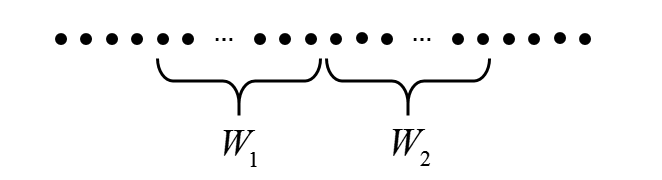
\includegraphics[width=0.4\textwidth]{img/sync_sliding_window.png}
			\caption{帧同步时滑动窗口示意图}
			\label{fig:sync_sliding_window}
		\end{figure}

		\begin{figure}
			\centering
			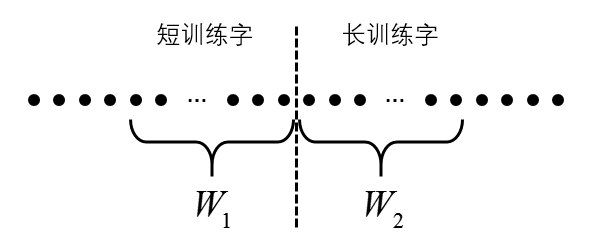
\includegraphics[width=0.4\textwidth]{img/sync_sliding_window_lts.png}
			\caption{符号同步时滑动窗口示意图}
			\label{fig:sync_sliding_window_lts}
		\end{figure}

	下面介绍如何添加同步相关性的软件接口,以互相关性为例介绍,自相关性与之类似。

	第一步,列出同步互相关性的公式,分析哪些计算适合由硬件完成,哪些计算适合引出到软件由软件完成。
	\ref{math:sync_inter_correlation}是互相关性的公式,其中$P_n$是归一化系数。
		\begin{equation}
			\centering
			C_n = \sum_{k=0}^{L-1} r_{n+k} \cdot s_{n+k}^*
		\end{equation}
		\begin{equation}
			\centering
			P_n = \sum_{k=0}^{L-1} |r_{n+k}|^2 \cdot \sum_{k=0}^{L-1} |s_{n+k}|^2
		\end{equation}
		\begin{equation}
			\centering
			M_n = \frac{|C_n|^2}{P_n}
			\label{math:sync_inter_correlation}
		\end{equation}

	我们知道FPGA硬件适合做乘法与加法,不适合做除法,除法需要多周期,延迟高。因此,我们可以把计算$C_n$与$P_n$交由硬件完成。
	另外,因为长训练字的能量值$\sum_{k=0}^{L-1} |s_{n+k}|^2$是固定的,我们只需在硬件中计算$\sum_{k=0}^{L-1} |r_{n+k}|^2$,称作$P'_n$,
	计算$M_n$的过程由软件完成。

	第二步,在同步模块内计算得到$C_n$、$P'_n$,并从同步模块引出。
	添加同步模块的端口,如下所示,这里只是示意代码,实际上除了$C_n$、$P'_n$外,我们还引出了计算自相关性的几个信号。
	\begin{lstlisting}[language={Verilog}]
module rx_synchronization(
... // other ports
input signal_valid,
output [31:0] sync_para_C,
output [31:0] sync_para_P1,
... // other ports
);
	\end{lstlisting}
	signal\_valid信号是指后续模块解出了signal字段,只有signal字段符合要求时此值为1,否则为0。
	我们在signal\_valid为1时为sync\_para\_C、sync\_para\_P1赋值。

	第三步,做时钟域转换,把同步模块对应时钟域下的sync\_para\_C、sync\_para\_P1,
	转化为AXI总线时钟域下的axi\_sync\_para\_C、axi\_sync\_para\_P1,并赋值给AXI寄存器。
	GRTSEC提供了一个时钟域转换模块reg\_clk\_domain\_switch,使用方法如下所示,我们将$C_n$、$P'_n$合并后一起转时钟。
	\begin{lstlisting}[language={Verilog}]
reg_clk_domain_switch_64 SEC_SYNC_clk_switch_clk0_to_clkaxi(
.clk_pre(usr_clk_ch0),
.clk_pos(S_AXI_ACLK),
.rst_pre(usr_rst_ch0),
.rst_pos(~S_AXI_ARESETN),
.reg_pre(sync_para),
.reg_pos(axi_sync_para)
);
	\end{lstlisting}

	第四步,从嵌入式软件代码读取$C_n$、$P'_n$,并用软件计算出我们所需的$M_n$。
	嵌入式软件读取和计算代码如下所示,SYNC\_PARA\_LTS为预存好的长训练字的能量值。
	\begin{lstlisting}[language={C}]
int syncParaC = Xil_In32(PHYSyncPara1);
int syncParaP1 = Xil_In32(PHYSyncPara2);
float syncParaM = syncParaC * syncParaC / (syncParaP1 * SYNC_PARA_LTS);
	\end{lstlisting}

	至此,以同步相关性为例,用户完成了物理层信息的扩展。

	\section{多射频模式}\label{sec:grtsec_loopback}
	在实际的WiFi安全使用样例设计中,我们发现一个问题,在真正通过空气进行通信之前,研究者往往会先验证数据处理流程是否能在硬件上正常工作,
	类似于将射频前端的发送端与接收端通过馈线相连,因此需要验证平台提供对完美信道进行模拟的能力,但原有的GRT2.0的射频通信库不支持这一点。
	完美信道是指将发送端和接收端之间连接在一起,接收到的信号与发送信号完全相同,
	用以验证物理层信息是否是完美信息,比如CSI全部为1,频偏为0,同步相关性为1等,
	以及模拟在完美通信时新数据处理算法是否可行,排除信号偏差带来的影响,
	比如验证加密解密算法在硬件上运行是否正确,不需要真正地与射频前端连接起来。

	为了支持完美信道,我们对射频通信库进行了扩展,提供两种模式,射频模式和回环模式。
	射频模式是原射频通信库采用的方式,与射频前端相连。回环模式是将发送数据直接反馈给接收端。

	这样做的好处是,WiFi安全的研究者在研究的前期系统实现与调试阶段,使用回环模式对完美信道进行模拟,
	不需要购买射频前端,不需要两台设备互相通信,便可以得到一些测试结果,对系统实现进行调试。
	搭配射频前端后,只需要修改一个参数,就能迅速适配射频前端,在空气中完成通信实验。

		\begin{figure}
			\centering
			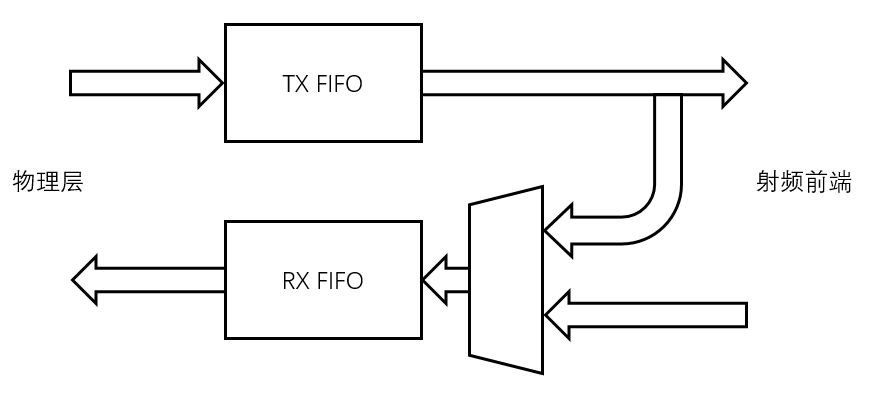
\includegraphics[width=0.7\textwidth]{img/rflib_loopback_mux.png}
			\caption{射频通信库射频模式与回环模式示意图}
			\label{fig:rflib_loopback_mux}
		\end{figure}

	下面介绍回环模式的具体实现,示意见图\ref{fig:rflib_loopback_mux}。
	射频通信库与物理层的数据接口是两个异步FIFO,在回环模式中,我们将发送端FIFO的输出,直接接到接收端FIFO的输入上。
	当有数据来时,向接收FIFO中填充空白信号,模拟空气中的无信号时的空白时间,当物理层发送端告知射频通信库要发送一帧时,
	进入回环模式,从发送端FIFO取数据,直接放到接收端FIFO中。

	值得注意的是,除了数据流需要做多路选择,时钟和复位信号也要做多路选择。
	收发FIFO都是异步FIFO,在射频模式时,射频端的时钟和复位信号来自射频模块,在回环模式时,需要改成物理层时钟,
	如下所示。
	\begin{lstlisting}[language={Verilog}]
assign clk = (MODE == RFD_MODE_LOOPBACK)? PHY_clk : rf_clk;
assign rst = (MODE == RFD_MODE_LOOPBACK)? PHY_rst : rf_rst;
	\end{lstlisting}

	\section{本章小结}\label{sec:grt2.0_summary}
	本节介绍了GRTSEC在GRT2.0系统上的改进,
	首先在\ref{sec:grtsec_overview}小节介绍了总体设计,
	面对GRT2.0嵌入式软件与物理层硬件交互不便,研究者无法通过软件获取物理层信息的问题,
	我们提出将物理层通过AXI总线与嵌入式处理器相连的解决方案,将物理层信息从硬件中提取出来,
	提供软件编程接口,并设计了一个硬件分析模块对安全研究进行支持,
	这样做的好处是方便WiFi安全的研究者获取常见的物理层信息,可以扩展其它物理层信息,可以使用硬件分析模块对算法进行加速。

	\ref{sec:grtsec_phyinfo_substract}小节介绍了CSI、频偏、RSSI、调制方式的提取方法,
	面对帧对齐和精确接收问题,我们采用物理层信息的三级缓存方法和添加时间戳的方法。
	\ref{sec:grtsec_phyinfo_api}小节介绍了物理层信息的软件接口,
	设计了嵌入式软件和主机软件的两级编程结构,满足了研究者在不同层编程的需求。
	\ref{sec:grtsec_phyinfo_analyzer}小节介绍了硬件分析模块的设计,
	提供了一个硬件分析模块对软件处理过程进行加速,适用于加密解密等计算密集的安全算法。
	\ref{sec:grtsec_phyinfo_extension}小节以同步相关性为例介绍了用户如何扩展物理层信息。
	\ref{sec:grtsec_loopback}小节介绍了为提高开发调试的效率,射频通信库模块增加回环模式,提供对完美信道的支持。
